\documentclass{beamer}
\mode<presentation>
{
  \usetheme{Warsaw}      % or try Darmstadt, Madrid, Warsaw, ...
  \usecolortheme{dolphin} % or try albatross, beaver, crane, ...
  \usefonttheme{structurebold}  % or try serif, structurebold, ...
  \setbeamertemplate{navigation symbols}{}
  \setbeamertemplate{caption}[numbered]
} 

\usepackage[english]{babel}
\usepackage[utf8x]{inputenc}
\usepackage{listings}
\usepackage{amssymb}
\usepackage{amsmath}
\usepackage{calrsfs}

%----------------------------------
% Fill in metadata
%----------------------------------

\title[Docker 101]{Hands-on with Docker}
\subtitle{\ldots part of an ELUG lecture series}
\author[B. Schafer]{Braxton Schafer} % between [] is short name, between {} is long name
\date{2019-10-28} % Here you can also just type something, e.g. October 10, 2017
\institute[Epic]{Epic - CaTS \\ Unix Engineer}

%----------------------------------
% ACTUAL PRESENTATION STARTS HERE
%----------------------------------

\begin{document}

% TITLE PAGE	
\maketitle
\addtocounter{framenumber}{-1} % We don't count the title page

% FRAME 1 
\section{Introduction \& Getting Started}
\subsection{What's a Docker?}
\begin{frame}[fragile]{Key Points}
\begin{itemize}
    \item Lightweight - base Ubuntu uses ~3MiB mem and no CPU.
    \begin{itemize}
    \item \texttt{docker stats}
    \end{itemize}
    \item Ephemeral
    \item Reproducible:
\end{itemize}
\begin{lstlisting}
FROM ubuntu
COPY . .
ENTRYPOINT /entrypoint.sh
\end{lstlisting}
\end{frame}
\begin{frame}{Containers vs. VMs}

\begin{figure}
\centering
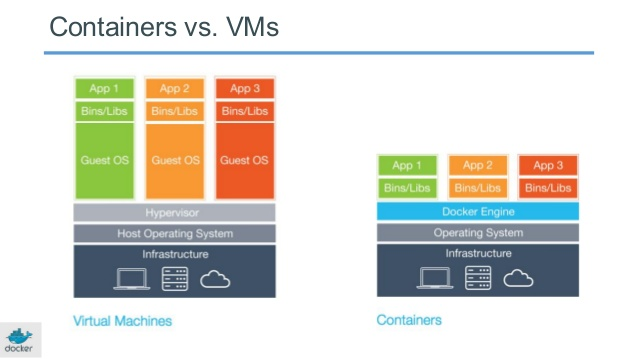
\includegraphics[width=10cm]{Pictures/container-vs-vms.jpg}
\caption{Courtesy docker.com}
\end{figure}

\end{frame}

\begin{frame}{What a Container Is Not}
   \begin{itemize}
       \item A security boundary
       \item Magical
       \item A panacea
   \end{itemize}{} 
\end{frame}

\subsection{Hands-On}

\begin{frame}[fragile]{Run Your First Container}
\begin{lstlisting}
$ docker pull ubuntu:18.04
$ docker create --name=babbys-first-container \
  --restart=unless-stopped \
  --interactive \
  --tty \
  ubuntu:18.04
$ docker start babbys-first-container
$ docker exec -it babbys-first-container /bin/bash

root@foobar:/# uname -a
\end{lstlisting}
\end{frame}

\section{Building Containers}

\subsection{Dockerfile}

\begin{frame}{Dockerfile}
\cdots
\end{frame}

\subsection{Layers}

\begin{frame}[fragile]{Layers}

\begin{itemize}
    \item Each command/line in a Dockerfile is a layer
    \item Best practice: Chain \texttt{RUN}s when possible:
    \begin{lstlisting}
    RUN apt-get update && \
        apt-get install foo bar baz && \
        foo --options
    \end{lstlisting}
\end{itemize}
    
\end{frame}

\section{Docker Internals}

\subsection{Kernel Stuff}

\begin{frame}{\texttt{cgroups} \& kernel namespaces}
\begin{itemize}
    \item Namespace kinds
    \begin{itemize}
        \item Mount
        \item Process
        \item Net
        \item IPC
        \item UID
    \end{itemize}
    \item \texttt{cgroups} (control groups)
    \begin{itemize}
        \item Restricts resource usage
        \item Prioritizes
        \item Accounting
        \item Control
    \end{itemize}
\end{itemize}
\end{frame}

\subsection{Containers}

\begin{frame}{\texttt{runc} \& \texttt{containerd} \& \texttt{dockerd} OH MY}
\begin{itemize}
    \item \texttt{runc} - interacts with cgroups and kernel namespaces
    \item \texttt{containerd} - bridge between \texttt{dockerd} and \texttt{runc}
    \item \texttt{dockerd} - interacts with userspace \texttt{docker} command
\end{itemize}
\end{frame}

\section{Lab}
\subsection{Database}
\begin{frame}[fragile]{\texttt{mysql}}
    \begin{lstlisting}
    $ docker create --name=mysql \
     --volume="$PWD/mysql-data":/var/lib/mysql \
     --env=MYSQL_ROOT_PASSWORD=foobar \
     --env=MYSQL_DATABASE=ghost
     --restart=unless-stopped \
     mysql:5
    $ docker start mysql
    $ docker logs mysql -f
    \end{lstlisting}
\end{frame}

\subsection{Inspecting}
\begin{frame}{Manipulating containers}
    \begin{itemize}
        \item \texttt{docker ps} - see running containers
        \item \texttt{docker ps -a} - see all containers
        \item \texttt{docker start/stop container-name} - start or stop a container
        \item \texttt{docker rm container-name} - delete a stopped container
    \end{itemize}
\end{frame}

\begin{frame}{Inspecting running containers}
   \begin{itemize}
       \item \texttt{docker inspect container-name}
       \item \texttt{docker inspect mysql | grep `"IPAddress"' | awk `\{print \$2\}'}
       \begin{itemize}
           \item Container DNS ``just works'' (if you do it right)
       \end{itemize}
   \end{itemize}
\end{frame}

\subsection{Ghost}
\begin{frame}[fragile]{Ghost}
\begin{lstlisting}
$ docker create --name=ghost \
  -v "$PWD/ghost-data":/var/lib/ghost/content \
  --env=database__client=mysql \
  -e database__connection__host=ip-address-from-last-step \
  -e database__connection__user=root \
  -e database__connection__password=foobar \
  -e database__connection__database=ghost \
  --link=mysql \
  --publish 8080:2368 \
  ghost:3
$ docker start ghost
$ curl http://localhost:8080
\end{lstlisting}
\end{frame}

\subsection{\texttt{docker-compose}}
\begin{frame}[fragile]{\texttt{docker-compose}}
https://pastebin.com/8vp9PSCw
\end{frame}

\subsection{Cleaning Up}
\begin{frame}{Cleaning Up}
    \begin{itemize}
        \item \texttt{docker rm -f \$(docker ps -qa)} -OR- \texttt{docker stop \$(docker ps -q) \&\& docker rm \$(docker ps -qa)}
        \item \texttt{docker system prune}
        \begin{itemize}
            \item Removes all stopped containers (like above)
            \item Removes unused images (\texttt{docker rmi \$(docker images -q)})
            \item Removes unused networks
            \item Removes dangling build cache
        \end{itemize}
        \item \texttt{docker \$component prune} - \texttt{docker volume prune} is another one.
    \end{itemize}
\end{frame}

\section{Wrap-Up}
\subsection{Resources/Cool Stuff}
\begin{frame}{Resources/Cool Stuff}
    \begin{itemize}
        \item https://hub.docker.com/\_/traefik - better ingress
        \item https://hub.docker.com - find all the images
        \item https://docs.docker.com/compose/compose-file/ - compose file reference
        \item https://docs.docker.com/engine/reference/builder/ - Dockerfile reference
    \end{itemize}
\end{frame}

\end{document}